\section{Government}
	\subsection{Registration}
	Government's account is only one because it has special privileges that
	they will explain later. For this reason, this account is provided 
	by the developer of \textit{Soldino}.
	\subsection{Login}
	If you want to log in with the government's account press the \texttt{login} button on the 
	top right of the homepage, you will automatically log in your account 
	(there is no need for a username or password, all data are done via MetaMask). 
	\\To be able to log in, make sure you are logged in with the correct MetaMask\glosp 
	account.
	\subsection{Logout}
	To log out of \textit{Soldino}, you just have to log out of 
	MetaMask\glosp. To do this, you have to press MetaMask's icon on the top 
	right of the browser, press your account's icon and then click on \texttt{Log out}
	on the top right.
	\begin{figure}[H]
		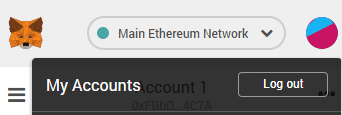
\includegraphics[width=7cm]{res/images/logout_metamask.png}
		\centering
		\caption{Logging out}
	\end{figure}
\pagebreak
	\subsection{Cubit}
	The government can mint and distribute Cubits\glosp by pressing the \texttt{Cubit 
	Manager} button in the navigation bar at the top of the page.
	\begin{figure}[H]
		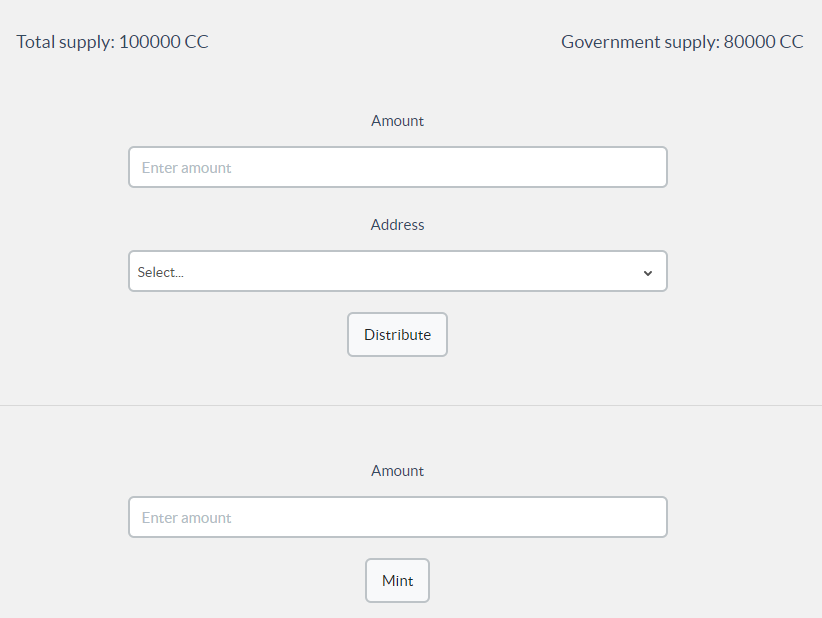
\includegraphics[width=15cm]{res/images/cubit_manager.png}
		\centering
		\caption{Goverment Cubit page}
	\end{figure}
		\subsubsection{Minting}
		To mint Cubits\glo{}, you have to insert the quantity you want in the 
		\texttt{Amount} field at the bottom of the page and then press \texttt{Mint}. Now you will 
		see that the \texttt{Government supply} is increased by the chosen amount.
		\begin{figure}[H]
			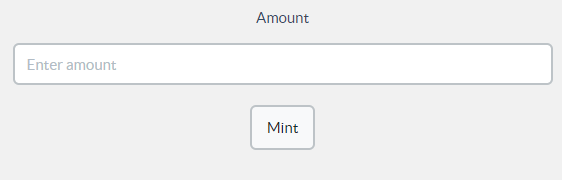
\includegraphics[width=15cm]{res/images/minting_cubits.png}
			\centering
			\caption{Minting Cubits}
		\end{figure}
		\subsubsection{Distributing}
		To distribute Cubits\glosp you have to insert the amount in the \texttt{Amount} 
		field and select the address of the accounts you wish to send the Cubits to 
		from the drop down menu. Every account you selected will have a checked 
		box next to their name. You can also search an account by name using the 
		specific search bar. When you are done press \texttt{Distribute}.\\

		\begin{figure}[H]
			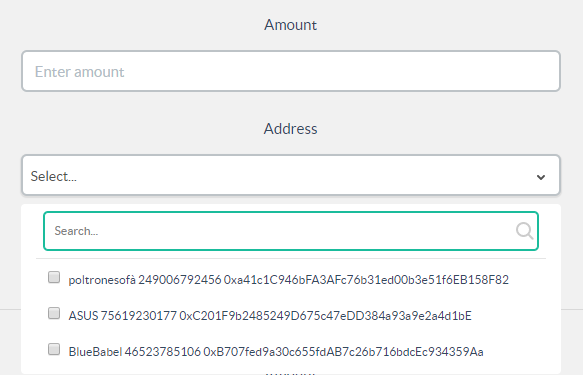
\includegraphics[width=15cm]{res/images/distributing.png}
			\centering
			\caption{Distributing Cubits}
		\end{figure} \mbox{}\\
		\noindent Note that the amount of cubits must be lower than the "Government  
		supply" otherwise you will not be able to send them.
	\subsection{Managing users}
	The Government can reactivate disabled accounts or deactivate active accounts.
	This can be done by clicking on the \texttt{Citizens List} or \texttt{Businesses List}
	in the navigation bar on the top of the page where all \textit{Soldino} users' information can be found.

	\begin{figure}[H]
		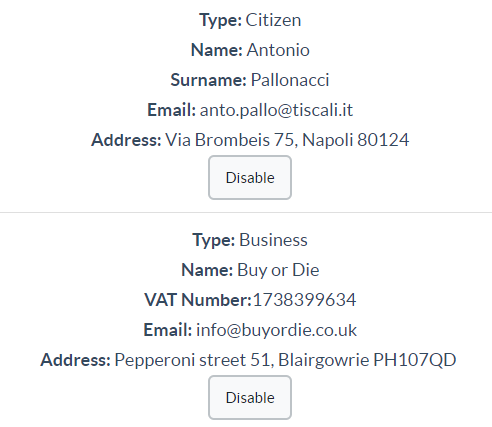
\includegraphics[width=13cm]{res/images/users_list.png}
		\centering
		\caption{Example of users list}
	\end{figure}
		\subsubsection{Deactivating users}
		Once you have found the account that you want to disable, press the 
		\texttt{Disable} button. Disabling an account means that it will no longer be able to make purchases on \textit{Soldino} 
		until it will be enabled again.

		\begin{figure}[H]
			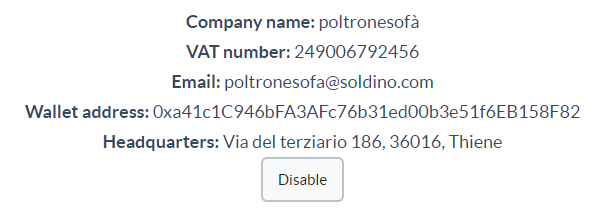
\includegraphics[width=15cm]{res/images/user_disable.png}
			\centering
			\caption{Example of disabling an activated account}
		\end{figure}
		\subsubsection{Activating users}
		Once you have found the account that you want to enable, press the button 
		\texttt{Enable}. After being enabled, an account can make 
		purchases on \textit{Soldino} again.
		\begin{figure}[H]
			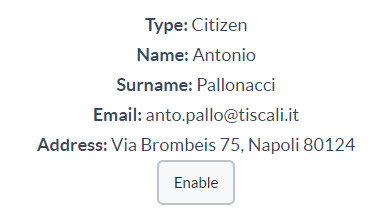
\includegraphics[width=15cm]{res/images/user_enable.png}
			\centering
			\caption{Example of enabling a deactivated account}
		\end{figure}
		
	\subsection{Refund VAT}
	To refund businesses of their VAT output, you have to press the \texttt{VAT 
	Refund} button in the navigation bar on the top of the page. In the 
	page that will be displayed, you will find all businesses with VAT output for the current quarter.
	Press \texttt{Refund} to refund the selected business.
	%After selecting the quarter you can search a Business by name and select 
	%them by status.
	%	CHE SIGNIFICA????
	\begin{figure}[H]
		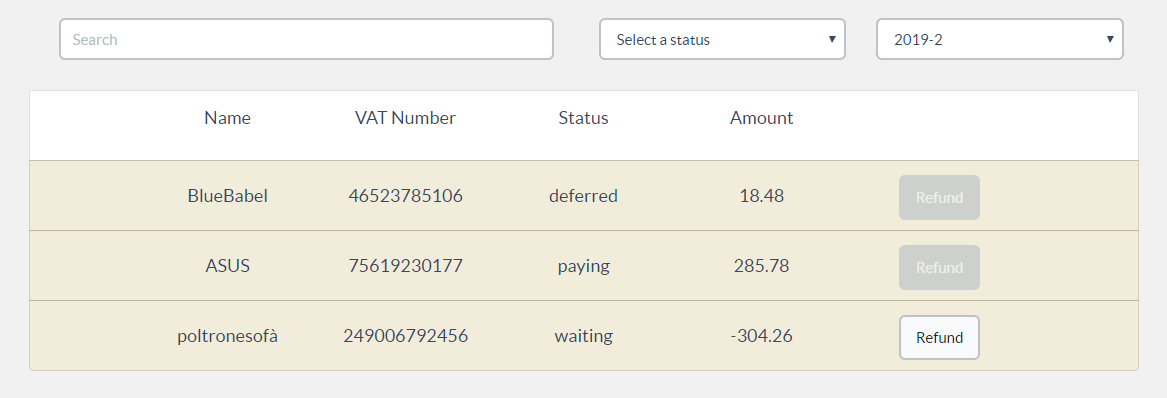
\includegraphics[width=15cm]{res/images/business_list.png}
		\centering
		\caption{List of Business}
	\end{figure}
	\noindent Press "Refund" to refund the selected business.\\
%	\begin{figure}[H]
%		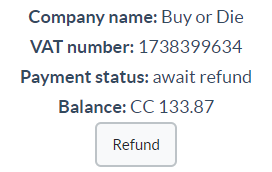
\includegraphics[width=7cm]{res/images/business_refund.png}
%		\centering
%		\caption{Example of reimbursing a business}
%	\end{figure}